
\documentclass[border=5pt]{standalone}
\usepackage[utf8]{inputenc}
\usepackage[T1]{fontenc}
\usepackage{amsmath,amssymb}
\usepackage{tikz}
\usetikzlibrary{arrows.meta,shapes.misc,calc}
\renewcommand{\familydefault}{\sfdefault}
\tikzset{
  ptcross/.style={cross out,draw,thick,minimum size=1.6mm,inner sep=0pt},
  vec/.style={->,thick,>={Stealth[length=2.6mm]}},
  vecu/.style={vec,color=blue!70!black},
  vecv/.style={vec,color=red!75!black},
  vecw/.style={vec,color=green!45!black},
  grid/.style={gray!35,thin},
}
\newcommand{\Vj}[1]{\overrightarrow{\text{#1}}}
\newcommand{\pt}[4]{\node[ptcross] at (#1,#2) {}; \node[anchor=#4,inner sep=2pt] at (#1,#2) {$#3$};}
\begin{document}
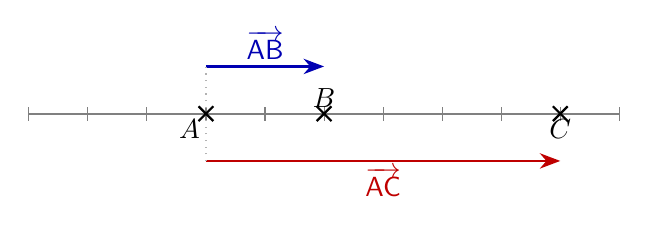
\begin{tikzpicture}[x=0.75cm,y=0.75cm]
\draw[thick,gray] (-3,0) -- (7,0);
\draw[gray] (-3,-0.12) -- (-3,0.12);
\draw[gray] (-2,-0.12) -- (-2,0.12);
\draw[gray] (-1,-0.12) -- (-1,0.12);
\draw[gray] (0,-0.12) -- (0,0.12);
\draw[gray] (1,-0.12) -- (1,0.12);
\draw[gray] (2,-0.12) -- (2,0.12);
\draw[gray] (3,-0.12) -- (3,0.12);
\draw[gray] (4,-0.12) -- (4,0.12);
\draw[gray] (5,-0.12) -- (5,0.12);
\draw[gray] (6,-0.12) -- (6,0.12);
\draw[gray] (7,-0.12) -- (7,0.12);
\draw[vecu] (0,0.8) -- (2,0.8) node[midway,above=1pt,inner sep=1pt] {$\Vj{AB}$};
\draw[vecv] (0,-0.8) -- (6,-0.8) node[midway,below=1pt,inner sep=1pt] {$\Vj{AC}$};
\draw[gray!60,dotted] (0,-0.8) -- (0,0.8);
\node[ptcross] at (0,0) {};
\node[anchor=north east,inner sep=2pt] at (0,0) {$A$};
\node[ptcross] at (2,0) {};
\node[anchor=south,inner sep=2pt] at (2,0) {$B$};
\node[ptcross] at (6,0) {};
\node[anchor=north,inner sep=2pt] at (6,0) {$C$};

\end{tikzpicture}
\end{document}
